%\chapter{Conception du projet}
%\label{sec:EnvironnementDeTravail}
\chapter{Analyse fonctionnelle et conceptuelle}
\label{sec:Analyse fonctionnelle et conceptuelle}
%Durant la réalisation de ce projet, nous avons essayé d’utiliser différents
%outils de développement, d’une part afin de rendre la tâche de la
%réalisation plus facile, d’autre part pour que notre système soit robuste et
%répond parfaitement a nos besoins , et que nos interfaces soient claires et
%faciles à utiliser.

%\section{Choix de langage de modélisation :}
\section{Analyse fonctionnelle}
%Dans cette section, je présente le langage et le logiciel de modélisation que j’ai utilisé pour concevoir notre solution.
\begin{comment}
	content...

\subsection{UML}
On a utilisé UML comme langage de modélisation.
Langage de modélisation unifié UML (Unified modeling Langage) un
consiste a modéliser une application logicielle d'une façon standard
dans le cadre de conception orientée objet.
UML consiste a couvrir le cycle de vie d'un logiciel depuis la
spécification des besoins jusqu'au codage en offrant plusieurs
moyens de description et de modélisation des acteurs.
\section{Choix de logiciel de modélisation :}
\subsection{Visual Paradigm  en ligne} 
Visual Paradigm  en ligne est un outil de création de diagrammes en ligne. Vous pouvez créer un nombre illimité de diagrammes, graphiques et autres visuels à partir d’un large éventail de types de diagrammes, y compris UML, organigrammes, BPMN, ERD, DFD, ArchiMate et autres.
%%%%%%%%%%%%%%%%%%%%%%%%%%%%%%%%%%%%%%%%%%%%%%%%%%%%%%%%% Tests %%%%%%%%%%%%%%%%%%%%%%%%%%
\section{Diagramme UML}
\begin{comment}
\begin{table}
		
	\caption{Rôles des diagrammes UML utilisés.}
	\label{table:kysymys}
\begin{tabular}{|c|p{11cm}|}
	
	\hline
	\large \bfseries Diagramme & \large \bfseries Rôle\\
	\hline
	Diagramme de cas d’utilisation & Il consiste à donner une vision globale sur les principales fonctionnalités
	(chaque fonctionnalité représente un cas d’utilisateur) d’une application .  \\
	\hline
	Diagramme d’activité &  Fournir une vue du comportement d'un système en décrivant la séquence d'actions d'un processus.    \\
	\hline
	Diagramme de séquence &Permettent d'identifier les classes requises par un système et le comportement des objets de classes au cours des interactions.  \\
	\hline
	Diagramme de classe    &Le diagramme de classes représente généralement un schéma utilisé en génie
	logiciel pour modéliser un problème bien précis, sous forme des classes et des
	interfaces ainsi que les différentes relations entre celles-ci. \\
	\hline
	
\end{tabular}

\end{table}
\end{comment}
%Table \ref{table:kysymys} on page \pageref{table:kysymys} refers to the ...
\newpage
\subsection{Diagramme de cas d’utilisation}
\begin{figure}[h!]
	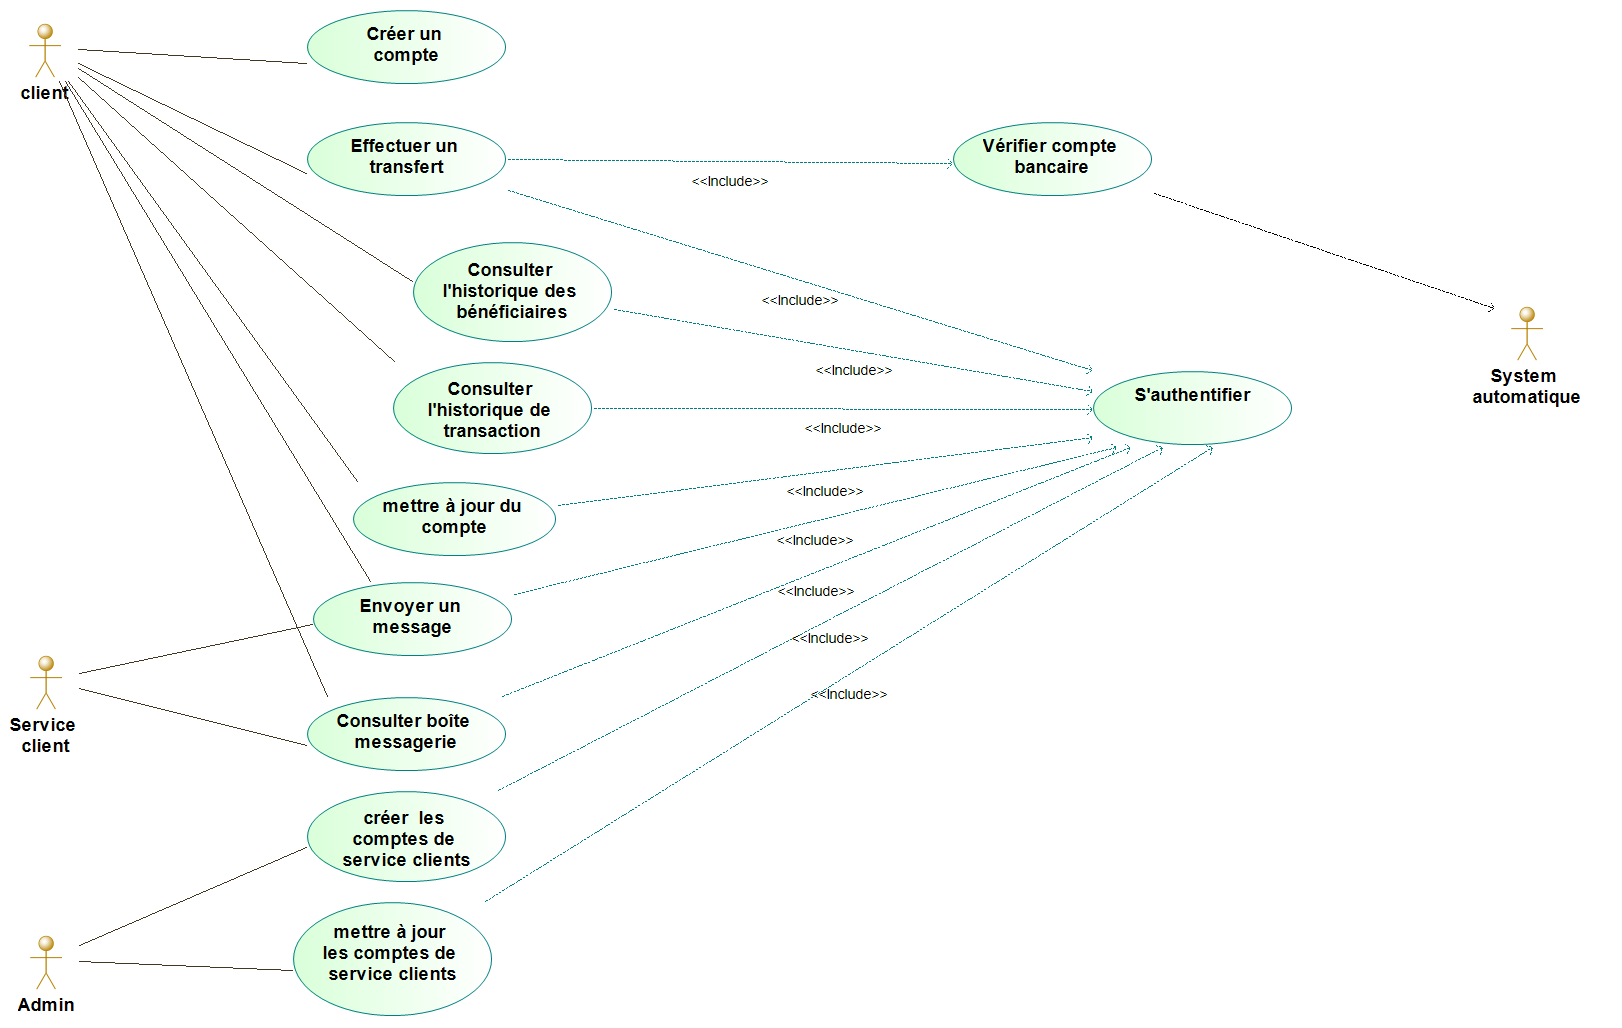
\includegraphics[width=18cm, height=21cm]{./Template LaTeX/Images/use_case.png}
	\caption{Diagramme de cas d’utilisation.}
	\label{fig1:use_case}
	
	
\end{figure}
\newpage
\subsection{Diagramme d’activité}
\subsubsection{Création de compte}
Le diagramme d’activité qu’illustre la figure~\ref{activiteCompte} décrit le cas d’utilisation « Créer un compte ».
\begin{figure}[h!]
	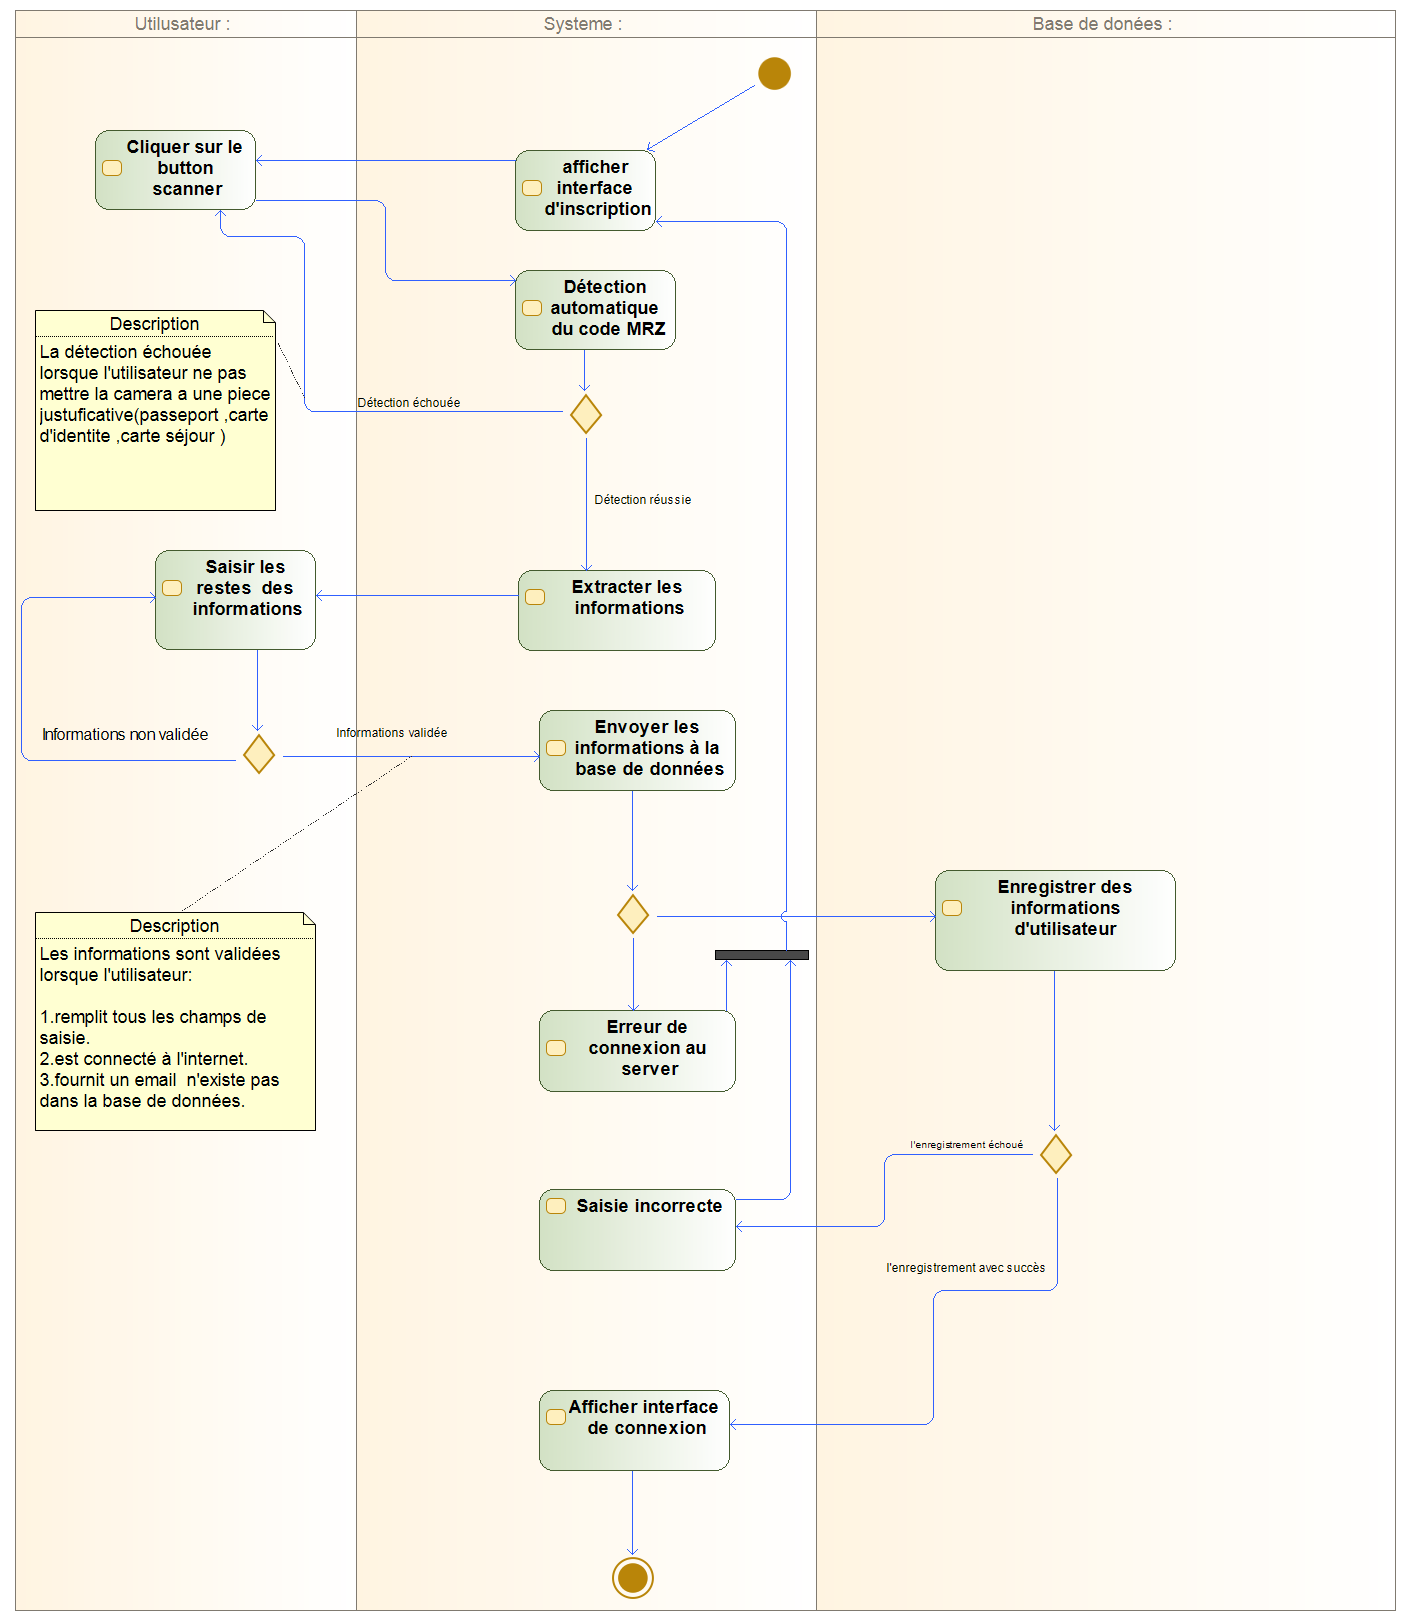
\includegraphics[width=18cm, height=19cm]{./Template LaTeX/Images/ins_act.png}
\caption{Diagramme d’activité : Création de compte}
\label{activiteCompte}

\end{figure}
\newpage
\subsubsection{Transfert d'argent}
Le diagramme d’activité qu’illustre la figure~\ref{activiteTr} décrit les différentes actions ou enchainements
effectués lors d’une opération de transfert d’argent.
\begin{figure}[h!]
	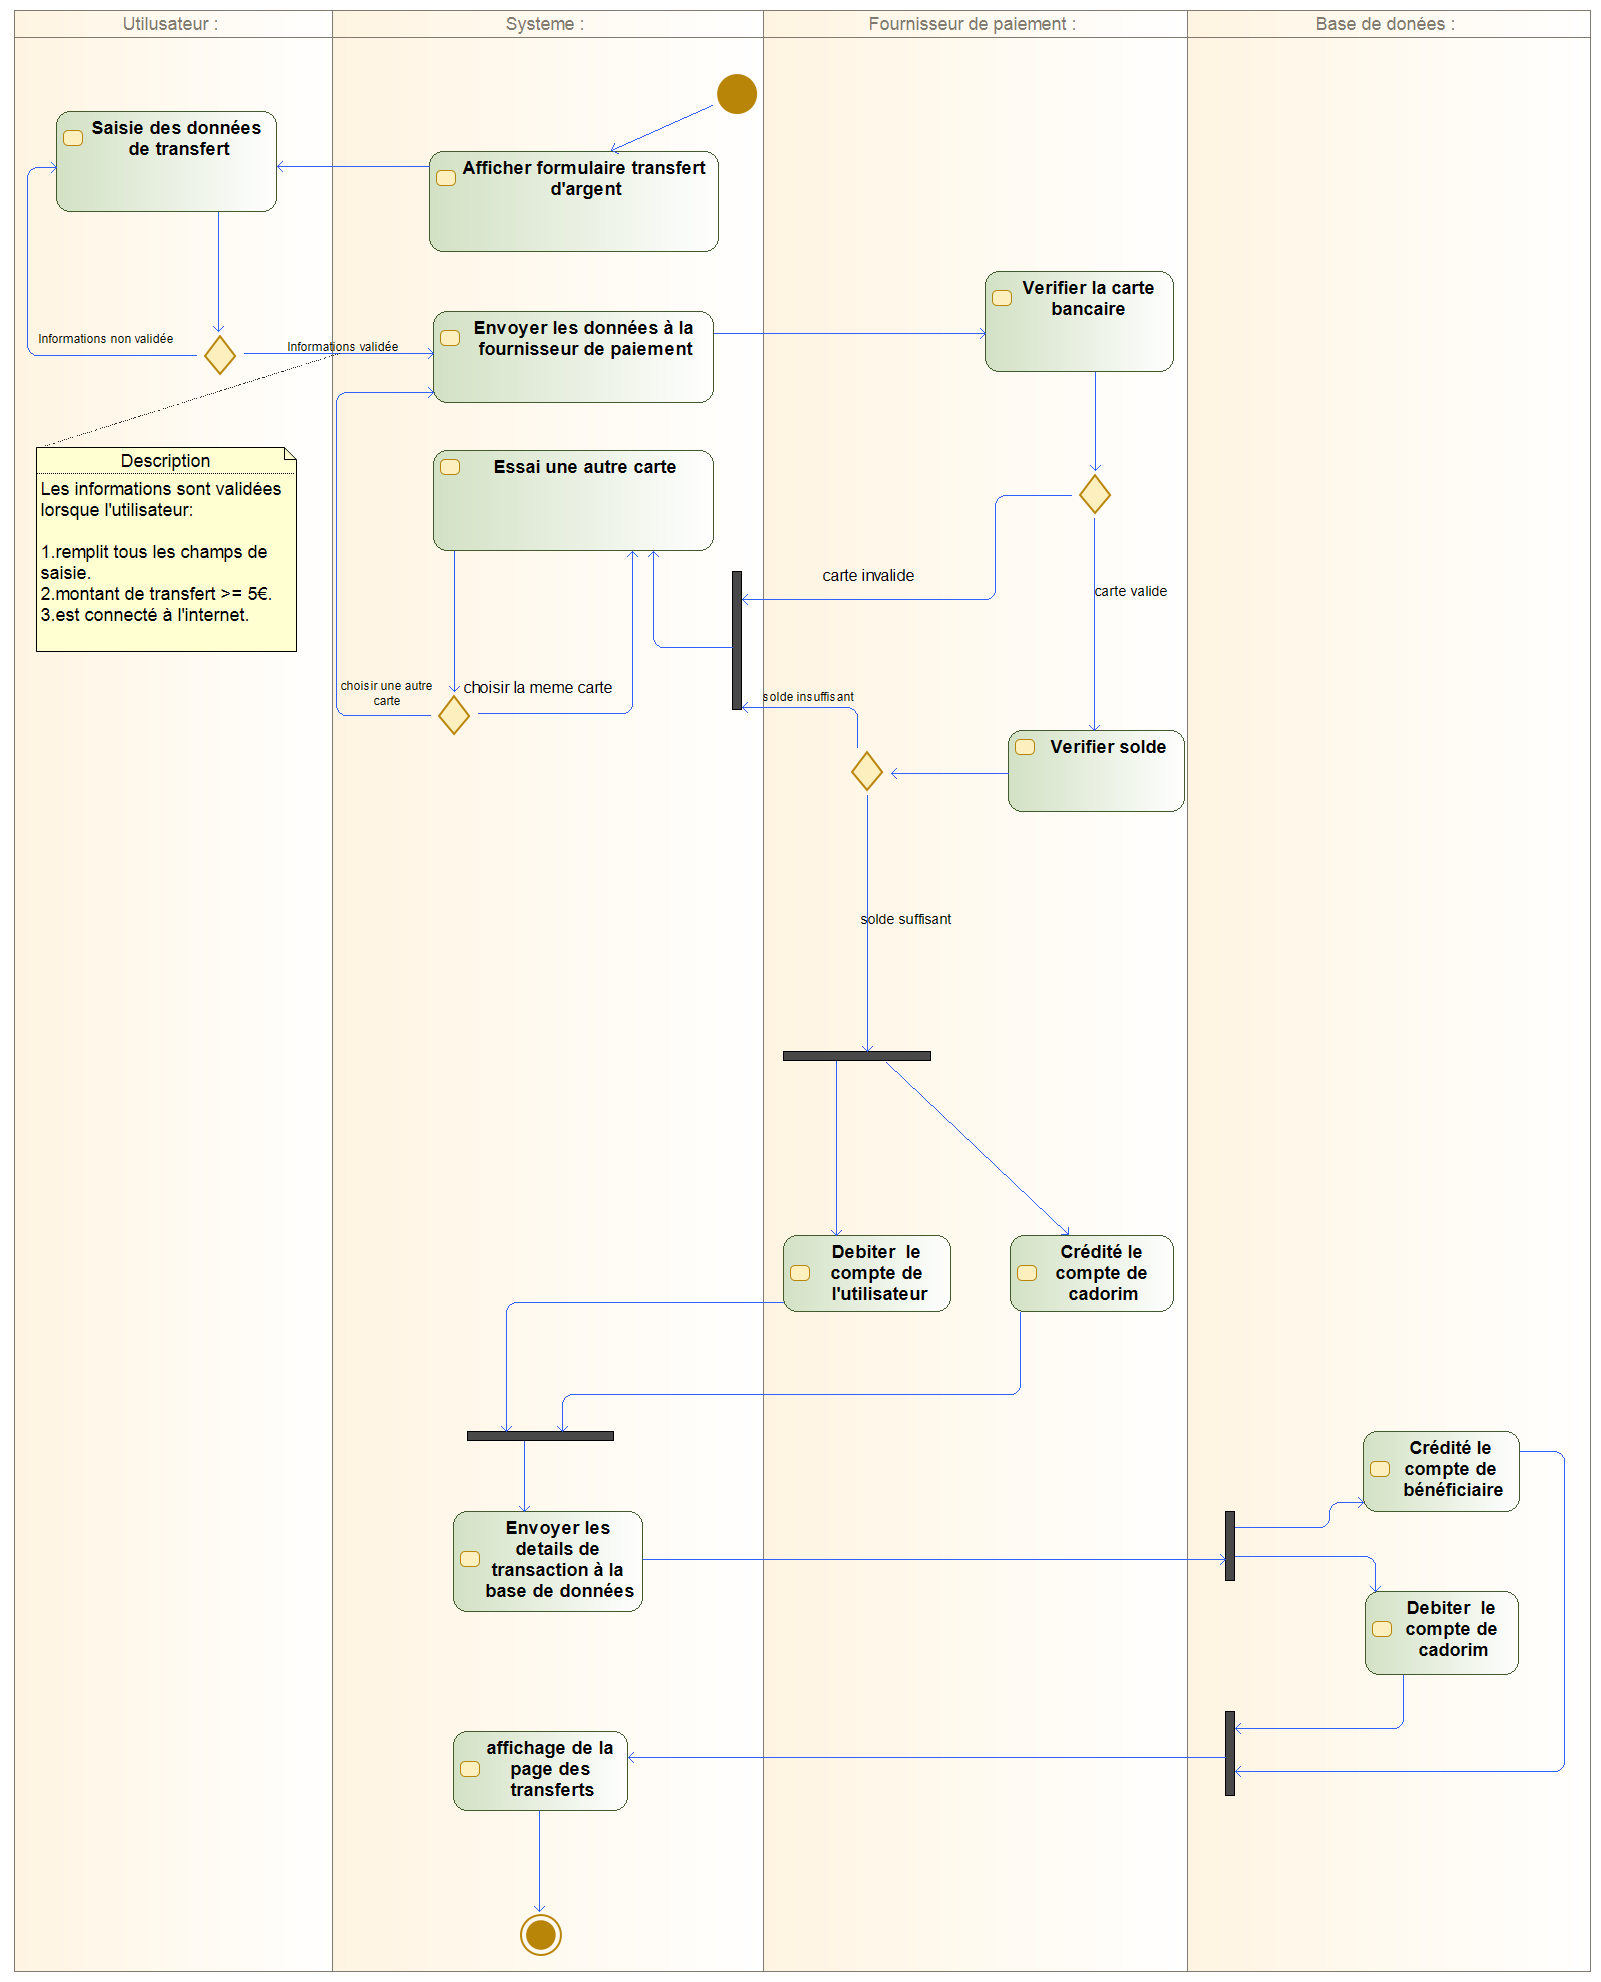
\includegraphics[width=18cm, height=20cm]{./Template LaTeX/Images/trans_act.png}
	\caption{Diagramme d'activité : Transfert d'argent}
	\label{activiteTr}
\end{figure}
\newpage
\subsubsection{Authentification}
Le diagramme d’activité qu’illustre la figure~\ref{activiteAuth} décrit le cas d’utilisation « Authentification ».
\begin{figure}[h!]
	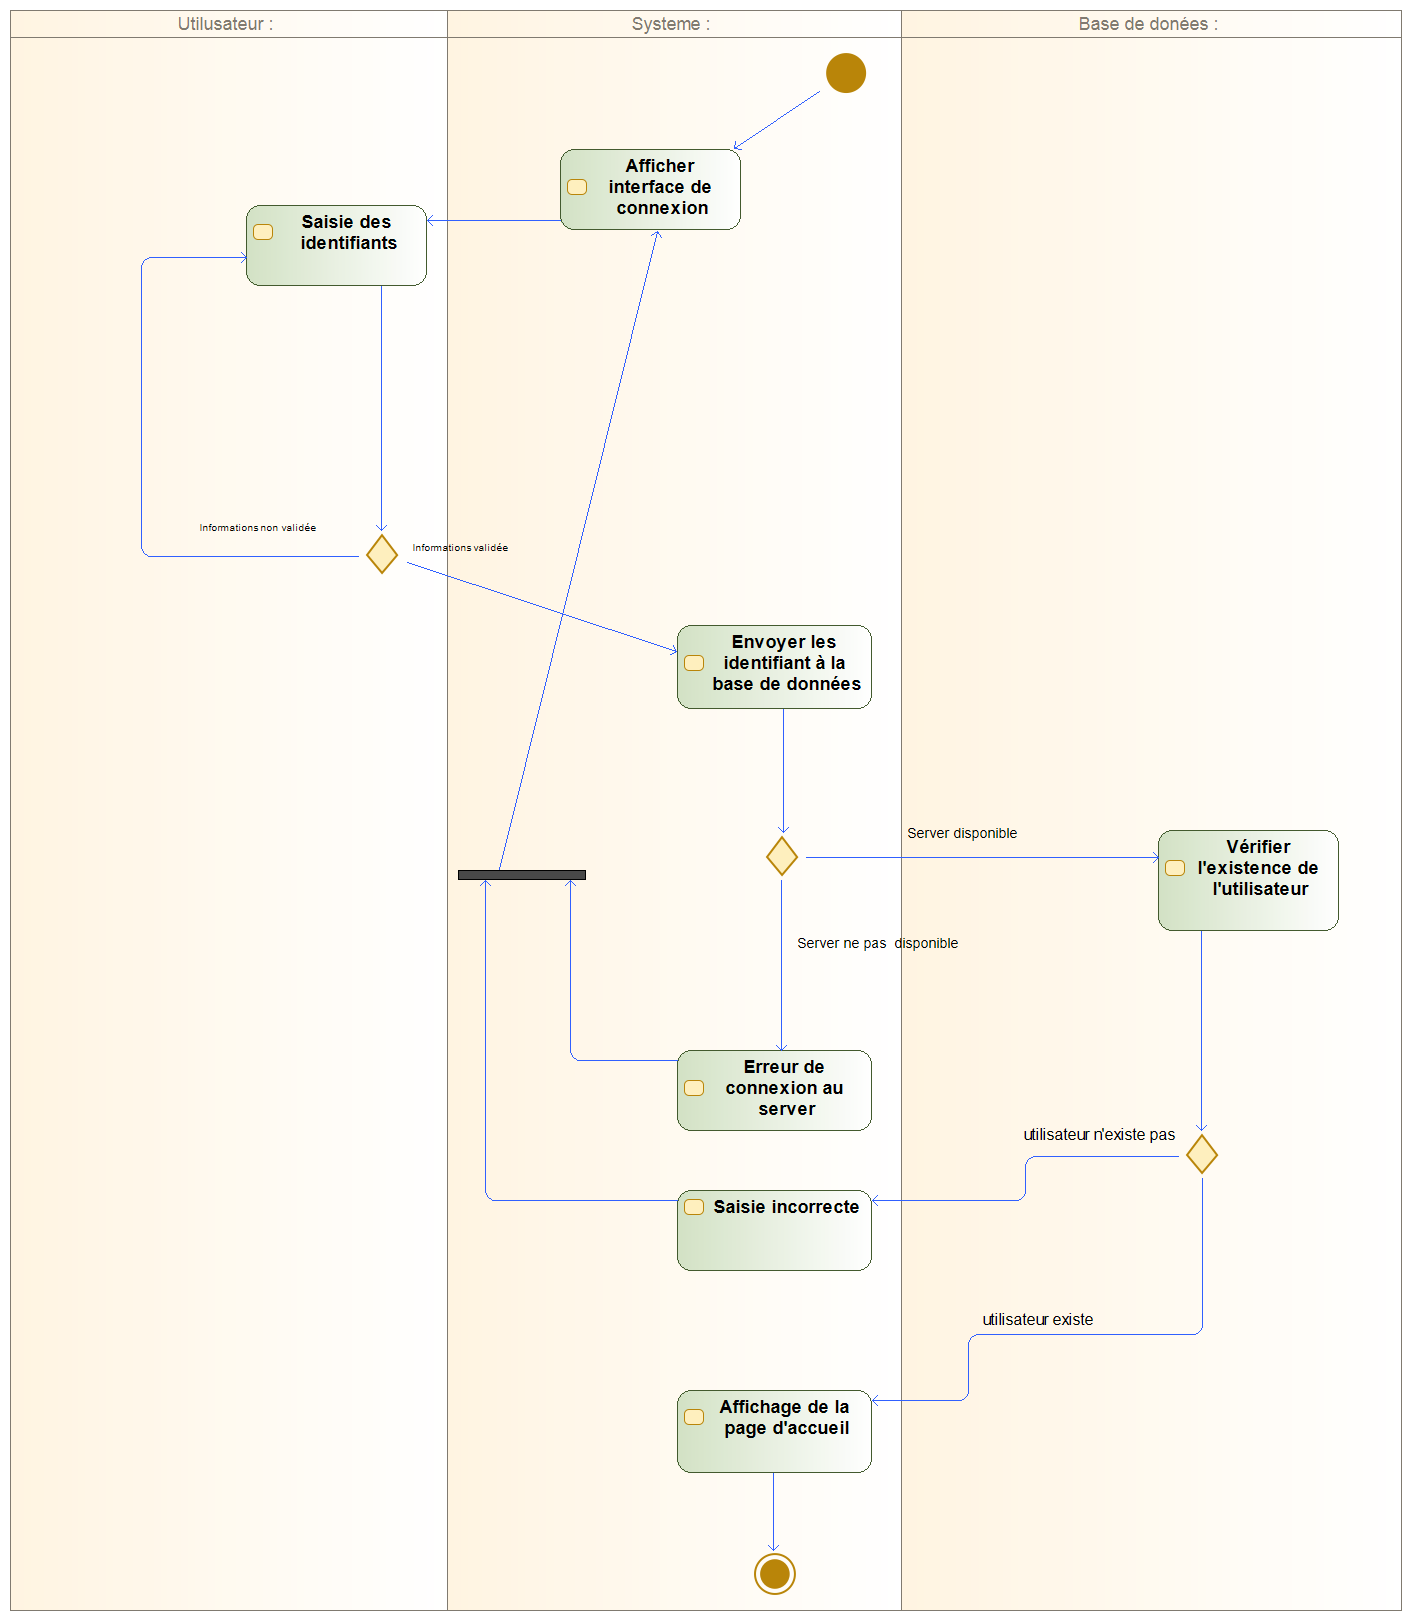
\includegraphics[width=18cm, height=20cm]{./Template LaTeX/Images/auth_act.png}
	\caption{Diagramme d'activité : Authentification}
	\label{activiteAuth}
\end{figure}


\section{Modélisation de la base de données}
%\subsection{Diagramme de séquence}
%\newpage
\subsection{Diagramme de classe}
\begin{figure}[h!]
	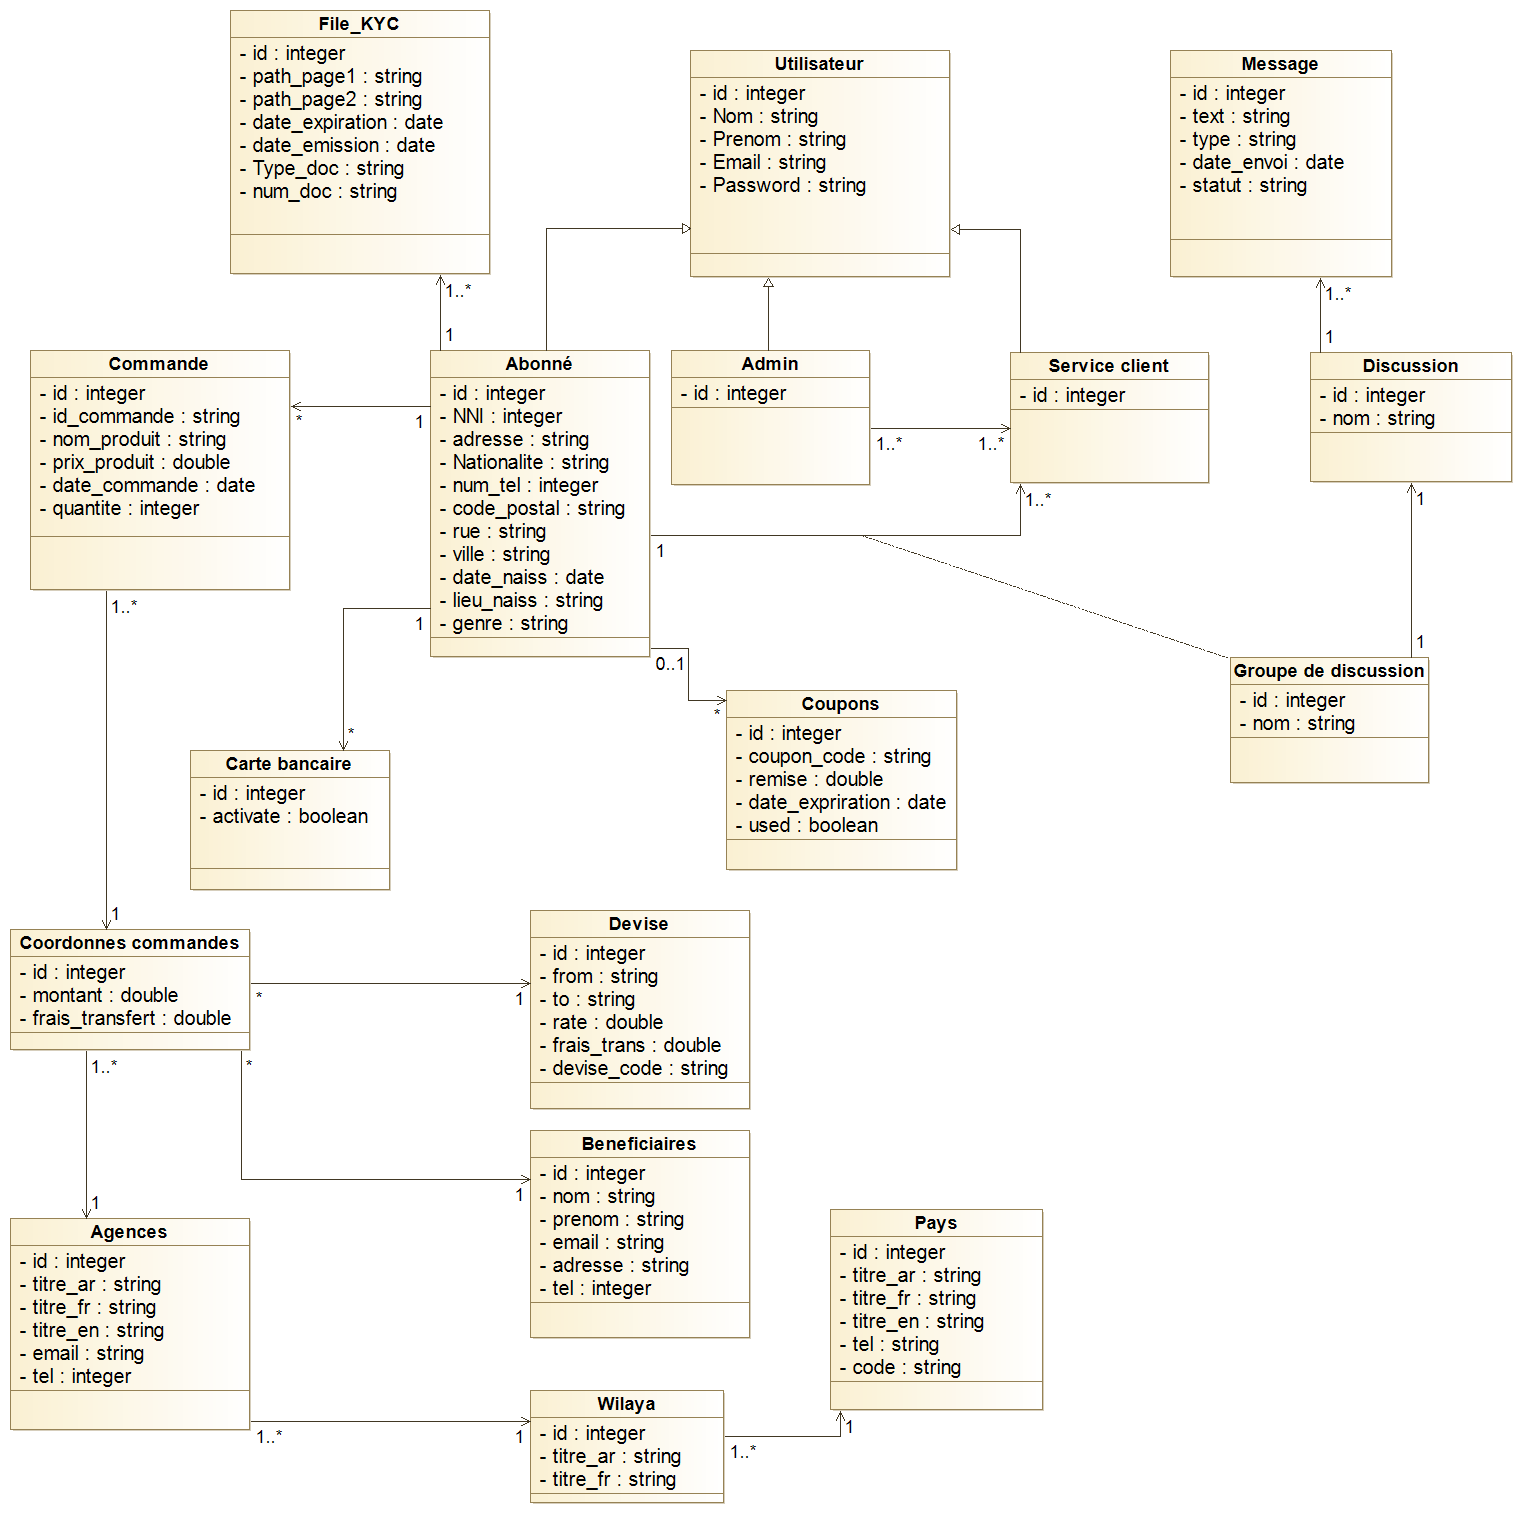
\includegraphics[width=18cm, height=20cm]{./Template LaTeX/Images/Diagramme_de_classe.png}
	\caption{Diagramme d'activité : Transfert d'argent}
	\label{fig4:class}
\end{figure}

%%%%%%%%%%%%%%%%%%%%%%%%%%%%%%%%%%%%%%%%%%%%5 ICI %%%%%%%%%%%%%%%%%%%%%%%%%%%%%%%%%%%%%%%%555

